\section{Versuchsaufbau/-durchführung}

Der Versuchsaufbau ist in Abbildung \ref{fig: versuchsaufabu} dargestellt.
\begin{figure}
  \centering
  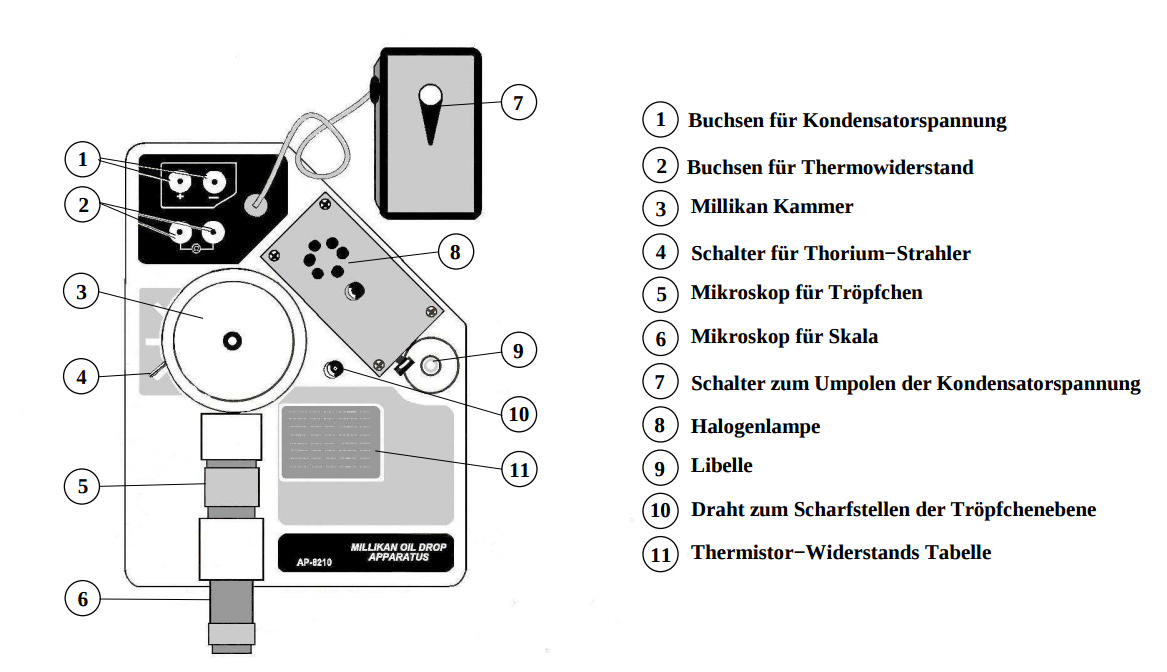
\includegraphics[width=0.6\textwidth]{pics/aufbau.png}
  \caption{Aufbau des Millikan-Versuches\cite{anleitung503}.}
  \label{fig: versuchsaufabu}
  \end{figure}
Die Öltröpfchen ($\rho\ua{oel}=\SI{866}{\kilogram\per\cubic\meter}$) werden in die Millikan-Kammer (\textbf{3}) zersteubt
und gelangen anschließend in den Kondensator. Der Abstand zwischen den Platten beträgt $d=\SI{7.6520}{\milli\meter}$.
Falls die Tröpfchen nicht durch die
Reibung geladen werden, kann mit Hilfe von (\textbf{4}) ein schwaches
$\alpha$-Präparat ($\ce{{232}^Th}\,8\,\mu\ce{Ci}$) die Tröpfchen ionisieren. Dazu
muss der Hebel (\textbf{4}) betätigt werden, um die Abschirmung zur Kammer
zu entfernen.

Die Öltröpfchen im Kondensator werden mit einem Mikroskop ((\textbf{5}) und (\textbf{6})) beobachtet,
die Lampe (\textbf{8}) liefert das dazu benötigte Licht.
Die am Kondensatorspannung anliegende Spannung ($U\in\left[0,301\right]\,\si{\volt}$)
wird mit einem Voltmeter so justiert, dass das Teilchen eine Schwebezustand erreicht.
Die Polung der Kondensatorspannung lässt sich mit dem Schalter (\textbf{7}) einstellen.

Zusätzlich wird die Temperatur in der Kammer für jede Messung dokumentiert, dazu befindet sich
ein Thermowiderstand im Kondensator. Auf Grund seines temperaturabhängigen Widerstandes, kann
damit, bei Messung des Widerstandes, die Temperatur bestimmt werden.

Die Messeapertatur muss in Waage stehen, dazu wird zur Justierung die
Libelle (\textbf{9}) verwendet.
Für ein Teilchen wird eingangs die Fallgeschwindigkeit $v_0$ bestimmt, dazu
wird die Zeit gemessen die ein Teilchen braucht, um eine Stecke von $s=\SI{0.5}{\milli\meter}$
zu durchlaufen. Anschließend schaltet man den Kondensator ein und stellt die Spannung
$U$ so ein, dass das Tröpfchen den Schwebezustand erreicht. Die eingestellte
Spannung wird notiert. Der Messvorgang wird mit dem aufschreiben des Thermowiderstands
abgeschlossen. Der Vorgang wird für 25 Öltröpfchen wiederholt.
